\def\year{2019}\relax
%File: formatting-instruction.tex
\documentclass[letterpaper]{article} % DO NOT CHANGE THIS
\usepackage{aaai19}  % DO NOT CHANGE THIS
\usepackage{times}  % DO NOT CHANGE THIS
\usepackage{helvet} % DO NOT CHANGE THIS
\usepackage{courier}  % DO NOT CHANGE THIS
\usepackage[hyphens]{url}  % DO NOT CHANGE THIS
\usepackage{graphicx} % DO NOT CHANGE THIS
\urlstyle{rm} % DO NOT CHANGE THIS
\def\UrlFont{\rm}  % DO NOT CHANGE THIS
\usepackage{graphicx}  % DO NOT CHANGE THIS
\frenchspacing  % DO NOT CHANGE THIS
\setlength{\pdfpagewidth}{8.5in}  % DO NOT CHANGE THIS
\setlength{\pdfpageheight}{11in}  % DO NOT CHANGE THIS

\usepackage[ruled, linesnumbered]{algorithm2e}
\usepackage{amsthm}

\newcommand{\inlinecite}[1]{\citeauthor{#1} \shortcite{#1}}

%PDF Info Is REQUIRED.
% For /Author, add all authors within the parentheses, separated by commas. No accents or commands.
% For /Title, add Title in Mixed Case. No accents or commands. Retain the parentheses.
% /Title ()
% Put your actual complete title (no codes, scripts, shortcuts, or LaTeX commands) within the parentheses in mixed case
% Leave the space between \Title and the beginning parenthesis alone
% /Author ()
% Put your actual complete list of authors (no codes, scripts, shortcuts, or LaTeX commands) within the parentheses in mixed case.
% Each author should be only by a comma. If the name contains accents, remove them. If there are any LaTeX commands,
% remove them.

% DISALLOWED PACKAGES
% \usepackage{authblk} -- This package is specifically forbidden
% \usepackage{balance} -- This package is specifically forbidden
% \usepackage{caption} -- This package is specifically forbidden
% \usepackage{color (if used in text)
% \usepackage{CJK} -- This package is specifically forbidden
% \usepackage{float} -- This package is specifically forbidden
% \usepackage{flushend} -- This package is specifically forbidden
% \usepackage{fontenc} -- This package is specifically forbidden
% \usepackage{fullpage} -- This package is specifically forbidden
% \usepackage{geometry} -- This package is specifically forbidden
% \usepackage{grffile} -- This package is specifically forbidden
% \usepackage{hyperref} -- This package is specifically forbidden
% \usepackage{navigator} -- This package is specifically forbidden
% (or any other package that embeds links such as navigator or hyperref)
% \indentfirst} -- This package is specifically forbidden
% \layout} -- This package is specifically forbidden
% \multicol} -- This package is specifically forbidden
% \nameref} -- This package is specifically forbidden
% \natbib} -- This package is specifically forbidden -- use the following workaround:
% \usepackage{savetrees} -- This package is specifically forbidden
% \usepackage{setspace} -- This package is specifically forbidden
% \usepackage{stfloats} -- This package is specifically forbidden
% \usepackage{tabu} -- This package is specifically forbidden
% \usepackage{titlesec} -- This package is specifically forbidden
% \usepackage{tocbibind} -- This package is specifically forbidden
% \usepackage{ulem} -- This package is specifically forbidden
% \usepackage{wrapfig} -- This package is specifically forbidden
% DISALLOWED COMMANDS
% \nocopyright -- Your paper will not be published if you use this command
% \addtolength -- This command may not be used
% \balance -- This command may not be used
% \baselinestretch -- Your paper will not be published if you use this command
% \clearpage -- No page breaks of any kind may be used for the final version of your paper
% \columnsep -- This command may not be used
% \newpage -- No page breaks of any kind may be used for the final version of your paper
% \pagebreak -- No page breaks of any kind may be used for the final version of your paperr
% \pagestyle -- This command may not be used
% \tiny -- This is not an acceptable font size.
% \vspace{- -- No negative value may be used in proximity of a caption, figure, table, section, subsection, subsubsection, or reference
% \vskip{- -- No negative value may be used to alter spacing above or below a caption, figure, table, section, subsection, subsubsection, or reference
\nocopyright
\setcounter{secnumdepth}{2} %May be changed to 1 or 2 if section numbers are desired.

% The file aaai19.sty is the style file for AAAI Press
% proceedings, working notes, and technical reports.
%

%%%%%%%%%%%%%%%%%%%%%%%%%%%%%%%
% Custom packages
\usepackage{tikz}
\usepackage{xcolor}
\usepackage{pgfplots}
\usetikzlibrary{positioning}
\usepackage{makecell}
\usepackage{listings}
\usepackage{subcaption}
%%%%%%%%%%%%%%%%%%%%%%%%%%%%%%%%

\def\HiLi{\leavevmode\rlap{\hbox to \hsize{\color{yellow!50}\leaders\hrule height .8\baselineskip depth .5ex\hfill}}}



%
% Add comments in the text
%
\newboolean{showcomments}
\setboolean{showcomments}{true}
%\setboolean{showcomments}{false}

\ifthenelse{\boolean{showcomments}}
  {\newcommand{\nb}[3]{
  {\color{#2}\small\fbox{\bfseries\sffamily\scriptsize#1}}
  {\color{#2}\sffamily\small$\triangleright~$\textit{\small #3}$~\triangleleft$}
  }
  }
  {\newcommand{\nb}[3]{}
  }

\newcommand\AF[1]{\nb{\textbf{Ariel:}}{red}{#1}}
\newcommand\Yossi[1]{\nb{\textbf{Yossi:}}{green}{#1}}
\newcommand\Roni[1]{\nb{\textbf{Roni:}}{blue}{#1}}



%\newcounter{definition}
\newtheorem{definition}{Definition}
\newtheorem{observation}{Observation}
\newtheorem{theorem}{Theorem}




\setlength\titlebox{2.5in} % If your paper contains an overfull \vbox too high warning at the beginning of the document, use this
% command to correct it. You may not alter the value below 2.5 in
\title{Solving the Longest Simple Path Problem With Heuristic Search}
%Your title must be in mixed case, not sentence case.
% That means all verbs (including short verbs like be, is, using,and go),
% nouns, adverbs, adjectives should be capitalized, including both words in hyphenated terms, while
% articles, conjunctions, and prepositions are lower case unless they
% directly follow a colon or long dash
\author{Submission \#59}
 \begin{document}

\maketitle

\begin{abstract}
The aim in the longest simple path (LSP) problem  is to find the longest simple path in a graph. LSP is a fundamental problem in graph theory with applications in a variety of domains including VLSI design, error correction code, and robot patrolling. This problem is known to be NP-hard. Prior approaches for solving LSP included using constraints solvers and genetic algorithms. However, very few works have applied systematic heuristic search techniques such as A*. In this work, we make several advancements towards solving the LSP problem with heuristic search.  First, we introduce several methods for pruning path prefixes that are dominated by others. Then, we propose several admissible heuristic functions for this problem, based on prior work on the snake-in-the-box problem. Experimental results demonstrate the large impact of the proposed heuristics and pruning rules.
\end{abstract}
\section{Introduction}

The longest simple path (LSP) problem is the problem of finding the longest simple path in a graph.
LSP is a fundamental problem in graph theory, that is known to be NP-hard, and even hard to approximate within a constant factor~\cite{karger1997approximating}. The motivation to solve the LSP problem comes from a variety of domains such as information retrieval on peer to peer networks \cite{Wong:2005:IRP:1062745.1062799}, estimating the worst packet delay of Switched Ethernet network \cite{DBLP:conf/sies/SchmidtS10}, multi robot patrolling \cite{Portugal:2010:MAM:1774088.1774360}, and VLSI design where the longest path should be found between two components on a printed circuit board \cite{chen2016vlsi}. Snake-in-the-box is a particular variant of LSP that is important for a useful type of efficient error correction codes~\cite{Kautz:1958:UDE}.




In this work we approach LSP as a heuristic search problem.
While there are many theory and algorithm for solving the shortest path problem, LSP was hardly studied as a search problem.
Indeed, there are several challenges in trying to solve LSP with heuristic search. In particular, the requirement that the solution path should be simple entails a blowup in the size of the search space. This is because a state represents a path and not a vertex.
Furthermore, in LSP we are looking for a solution with the maximal cost not the minimal cost. Thus, applying heuristic search for such problems is not trivial~\cite{DBLP:conf/socs/SternKPFR14}.


To address this, we propose several methods to detect and prune states that are \emph{dominated} by other states. We define this notion of domination between states formally, and provide two techniques for identifying when a state is dominated by another. We then show how to integrate these pruning methods into A* and into Depth-First Branch-and-Bound (DFBnB).

Then, we propose several admissible heuristics for LSP. This is especially challenging because most prior work in developing heuristics have been on minimization problems and on finding shorter paths. Finally, we perform a comprehensive set of experiments over grid map domains. Our results show that while some pruning is always useful, more sophisticated pruning is sometimes not worthwhile.

Several approaches where proposed for solving the LSP problem.
Some prior work compiled a given LSP problem to a constraint optimization problem and used a constraints solver~\cite{DBLP:conf/cpaior/PhamD12}. Others used genetic algorithms~\cite{DBLP:conf/smc/PortugalAR10}. While LSP in general is NP-Hard, it can be solved in polynomial time for certain classes of graphs~\cite{KeshavarzKohjerdi2012ALA}.
To the best of our knowledge, only two prior works approached LSP as a heuristic search problem. Palombo et al.~\shortcite{DBLP:conf/socs/PalomboSPFKR15} proposed several admissible heuristics for solving the snake in the box (SIB) problem, which is a special case of LSP. We build on these heuristics, adapted them to LSP, and propose novel heuristics as well as pruning techniques.
\inlinecite{DBLP:conf/socs/SternKPFR14} focused on general maximization problem and how to adapt heuristic search algorithms to solve them, and used LSP as a domain to demonstrate their results. Using a combination of our novel pruning techniques and heuristics, we are able to improve on their results by a up to a factor of 20.


%is related to solving a specific LPP - the Snake in the Box problem \cite{DBLP:conf/socs/PalomboSPFKR15}. Regardless of the above, our main motivation was pure curiosity.




% Much work on shortest path

% Key performance improvements: duplicate detection and heuristisc

% LSP is an important problem. A bit on prior work.
% But how to get heuristics and how to detection duplicate
% We detect dominating path
% We propose new heuristics
% We show they work experimentally



\section{Background}

%State space search is a general and popular problem solving method in which the problem is formulated as a a problem of finding a path or a vertex in a graph that repres In state space search, the problem  that has been applied


% State space search
\emph{State space search} algorithms are defined with respect to a \emph{state space}.
They are given (1) an initial state,
(2) a set of operators that define how to move from one state to another, and (3) a goal condition that defines which states are goal states. The output of a state space search algorithm is a path, i.e., a sequence of operators, from the initial state to a goal state.
In general, each state transition operator $o$ is associated with a cost denoted $cost($o$)$, and the cost of a path is the sum of costs of its constituent operators. For ease of exposition, we will assume in this paper that the cost of all operators is one, and so the length of a path corresponds to its cost. %


% Solving SP with state space search
A natural and common application of state space search algorithms is the well-known  shortest path (SP) problem. The SP problem is defined w.r.t a directed graph $G=(V,E)$, a start vertex $s\in V$, and a goal vertex $g\in V$.
A solution to a SP problem is a path in $G$ from $s$ to $g$ such that no other path from $s$ to $g$ is shorter. The corresponding state space is defined as follows: a state represents a vertex in $V$, the initial state is $s$, the state transition operators correspond to out-going edges, and the goal state represents the vertex $g$.

%a state is a path from $s$ to some vertex $n\in V$. The initial state is an empty path containing only $s$. The state transition operators correspond to adding an edge to a path. A goal state is a path from $s$ to $g$.





\subsection{A*}

%\AF{I think the description of A* is too long. Everybody knows A*. But, so be it.}
% Solving SP with A*: pruning paths and admissible heuristics
The A*~\cite{hart1968formal} algorithm is a popular state-space search algorithm that is often used to solve SP problems.
A* maintains two lists of states called OPEN and CLOSED.
For every generated state, A* maintains the length of the shortest path found so far from $s$ to that state. The latter is referred to as the $g$ value of that state. A* starts by adding the initial state to OPEN and setting its $g$ value to zero.

In every iteration, a state $n$ is popped out of OPEN and moved to CLOSE. Then, every applicable state transition operator is applied to $n$. This results in a set of states, one per applicable operator. This process is referred to as \emph{expanding} $n$ and the resulting set of states are referred to as the child states of $n$.
Every child state $c$ that was not generated before is added to OPEN, and its $g$ value is set to  $g(n)+$cost$(o)$, where $o$ is the operator applied to $n$ to generate $c$.
In some state spaces, there can be multiple paths to the same state.
This may cause a state $c$ to be generated more than once.
In such a case, when expanding a state $n$ and generating a child state $c$, it may be the case that $c$ is already in OPEN or CLOSED, and already has a $g$ value.
When this occurs, A* checks if its current $g$ value is smaller than or equal to $g(n)+cost(o)$. If it is, then $c$ is not inserted again to OPEN. Otherwise, the $g$ value of $c$ is updated to be
$g(n)+cost(o)$, and it is re-inserted to OPEN, removing the older copy of $c$ if it is in OPEN (it may already be in CLOSED).
This mechanism for keeping only the shortest path to each state is referred to as \emph{pruning dominating paths} or \emph{duplicate detection}, and is known to be very important in terms of runtime in some domains. Thus, many heuristic search algorithms implement pruning dominating paths mechanisms.


To choose which state to pop from OPEN in every iteration, A* uses a \emph{heuristic function}, denoted $h$, that estimates the length of the shortest path from a given state to a goal state. If that heuristic function never over-estimates the length of the shortest path to a goal then it is called an \emph{admissible} heuristic function. A* chooses in every iteration to pop the state $n$ in OPEN with the lowest $g(n)+h(n)$ value. If $h$ is an admissible heuristic, then when a goal state is expanded it is guaranteed that the lowest cost path to a goal has been found, and A* halts. Powerful admissible heuristics have been proposed over the years for a wide range of problems, and  having a strong heuristic function can lead to orders of magnitude speedup.


\subsection{Depth-First Branch-and-Bound (DFBnB)}
DFBnB is a simple search algorithm: it performs a depth-first search, keeps track of the cost of the best solution found so far,
and prunes any path in the state space that is more costly than the cost of the incumbent solution.


DFBnB can be coupled with an admissible heuristic, pruning every state $n$ for which $g(n)+h(n)$ is equal to or greater than
the cost of the incumbent solution. DFBnB is an anytime algorithm, and the solution it returns after pruning all branches in the state space is guaranteed to be optimal.

%\Roni{Hmm, should I add the psuedo code here or later? TBD}
%\Yossi{IMHO we can say that it is similar to the A* modifications - skip that}


\section{The Longest Simple Path Problem}
% LSP, definition
A path in a graph is called \emph{simple} if it never passes through the same vertex twice. Note that every solution to a SP problem must be simple, as otherwise a shorter path would exist.\footnote{This is not true if state transition operators can have zero or negative cost.} Thus, there is no meaningful difference between the SP problem and the problem of finding the shortest simple path. This is not the case for the problem of finding the \emph{longest} path: finding the longest path in a graph can be done in time that is polynomial in the number of graph vertices while finding the longest simple path is NP-Hard~\cite{karger1997approximating}.


% Problem definition
\begin{definition}[The longest simple path problem]
The Longest Simple Path (LSP) problem is defined w.r.t a directed graph $G=(V,E)$, a start vertex $s\in V$, and a goal vertex $g\in V$. A solution to LSP is a simple path from $s$ to $g$ such that no other simple path from $s$ to $g$ is longer.
\end{definition}

%\section{Heuristic Search for solving LSP}
% Maximization, challenges
In this work we explore how to apply heuristic search algorithms to solve the LSP problem.
In particular, we focused on two popular heuristic search algorithms: A* and DFBnB with a heuristic.


% State space formulation
To use A* or DFBnB to solve an LSP problem, one needs to first define a corresponding state space. For an SP problem, a state represented a vertex. This is not sufficient for LSP, since to know which operators are applicable in a vertex $n$ one must know the vertices in the path from $s$ to $n$ so as to make sure they are not added twice the resulting path.
%\Roni{Add an example of two paths to the same vertex, where there is a way to extend the paths but only one of the paths can do it without breaking the simple path requirement.}
Thus,
following Stern et al.~\shortcite{DBLP:conf/socs/SternKPFR14}, we define a state in the LSP state space to represent a path in the underlying graph $G$ from $s$ to a vertex $n$.\footnote{The initial state, which in LSP will be an empty path with one vertex -- $s$.}
To distinguish between a path in the underlying graph $G$ and a path in the LSP state space,  we will refer to the former as a \emph{graph-path}, and for an LSP state $N$
we use $N.\pi$ to denote its corresponding graph-path.
The applicable state transition operators from an LSP state $N$ correspond to extending
$N.\pi$ by extending it with a single edge.
%a graph-path from $s$ to $n$ by adding an out-going edge to $n$.
%applicable in a state representing a path that ends in a vertex $n$ are all ways to extend the corresponding graph-path by adding an edge to $n$ without violating the simple path requirement.


\subsection{A* and DFBnB for LSP}
LSP is a maximization (MAX) problem: the objective is to find the graph-path with the  maximal length. In general, some modifications to textbook A* are needed in order to make it compatible to MAX problems~\cite{DBLP:conf/socs/SternKPFR14}. These modifications include changing the definition of admissibility and changing how A* choose which state to pop from OPEN in every iteration.
\begin{itemize}
    \item \textbf{Admissibility in MAX problems.} A function $h$ is said to be admissible for MAX problems iff for every state $N$ in the search space it holds that $h(N)$ is larger than or equal to the length of the longest simple graph-path from $n$ to $g$.
    \item \textbf{Choosing from OPEN.} In MIN problems, A* pops from OPEN in every iteration the state $n$ with the lowest $g(N)+h(N)$. In MAX problems, A* needs to pop from OPEN in every iteration the state $N$ with the highest $g(N)+h(N)$.
\end{itemize}

In general MAX problems, there is third change that needs to be done to A* so that it works for MAX problems --- changing the stopping condition. In MAX problems, it may be the case that the optimal solution is to reach one goal state and continue the path to reach another (e.g., to gain more reward). Thus, expanding a goal is not a sufficient condition to guarantee optimality~\cite{DBLP:conf/socs/SternKPFR14}. However, in LSP this modification is not needed because there is a single goal vertex $g$ and since a solution must be a simple path we know that every optimal solution to LSP is a path that reaches the goal vertex exactly once and as the last vertex it visit.


The changed required to make DFBnB return optimal solutions for MAX problems are simple and very similar to the changes detailed above for A*:
(1) an admissible heuristic must now be an upper bound on the cost to go, and (2) a state $N$ can be pruned only if $g(N)+h(N)$ is smaller than or equals to the cost of the incumbent solution~\cite{DBLP:conf/socs/SternKPFR14}.


\subsection{Challenges}
Using either A* or DFBnB to solve LSP is not trivial, and raises several major challenges.
\subsubsection{State space size}
The size of the LSP state space is much larger than the SP state space defined over the underlying graph $G=(V,E)$: the SP state space is linear in $|V|$ while the LSP state space can be exponential in $|V|$.
For example, consider an empty $X\times Y$ grid, where $s$ is the grid cell in bottom-left and $g$ is the grid cell on the top-right.
The SP state space has $X\times Y$ states while the number of possible graph-paths from $s$ to $g$ is exponential in $X$ and $Y$.

%The huge size of this LSP state space emphasizes the need for an effective heuristic search algorithm to solve this problem. In this work we focused on two popular heuristic search algorithms: A* and Depth-first branch-and-bound (DFBnB).

\subsubsection{No pruning of dominated paths}
% No pruning
By construction, the LSP state space is a tree. Thus, there is exactly one path to reach each state, and consequently the duplicate detection mechanism used by A* and other algorithms will never detect a duplicate state. To address this, in Section~\ref{sec:prunning} we propose more aggressive path pruning mechanisms that is able to prune states in the LSP state space.


\subsubsection{Heuristics for Maximization Problems}
Most prior work in developing admissible heuristics have been for MIN problems. Standard techniques such as pattern database~\cite{culberson1998pattern,felner2004additive,edelkamp2014planning,haslum2007domain},  delete relaxation~\cite{hoffmann2001ff}, true distance heuristics~\cite{sturtevant2009memory,goldenberg2010portal} are all designed for MIN problems. The field of heuristic search has largely neglected the theory and practice of developing heuristics for MAX problems, and thus developing effective admissible heuristic for LSP is a challenge. We meet this challenge in Section~\ref{sec:heuristics}.





\section{Pruning Dominated States}
\label{sec:prunning}


Let $f^*(N)$ denote the length of the longest path from $s$ to $g$ that is an extension of $N.\pi$,
that is, the length of the longest path that starts with $N.\pi$ and ends at $g$.
We say that a state $N$ \emph{dominates} a state $N`$ iff
$f^*(N)\geq f^*(N`)$.
%\AF{Not clear. Who is a prefix of who. Please reword. This is importsant because this dominating attribute is used below} \Roni{OK}
Clearly, any search algorithm that aims to solve LSP can safely prune $N`$. In this section, we introduce several methods to identify this dominance relation between states, and show how to use these methods in A* and in DFBnB.


\subsection{Basic Symmetry Detection}
For an LSP state $N$ we introduce the following notation:
(1) $N.head$ is the last vertex in $N.\pi$,
and (2) $N.tail$ is all other vertices in $N.\pi$.
We say that that two states are {\em symmetric} if their heads are in the same location and their tail covers exactly the same set of cells, not necessarily in the same order. Figure~\ref{bsd-example} shows an example of two symmetric paths.
\begin{observation}
For every pair of symmetric states $N$ and $N`$, it holds that $N$ dominates $N`$ and vice versa.
\label{obs:symmetry}
\end{observation}
A direct corollary from Observation~\ref{obs:symmetry} is that if a search algorithm generates two symmetric states, it can safely prune one of them. We call to this dominance detection method the {\em Basic Symmetry Detection} (BSD) method.

\begin{figure}[ht!]
  \centering
  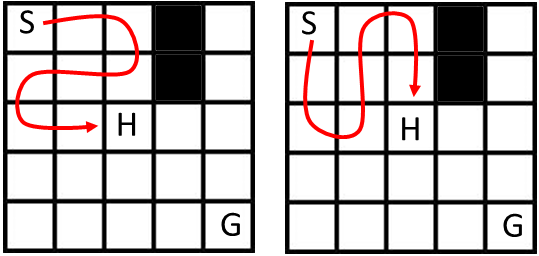
\includegraphics[width=2.7in]{fig/bsd-example.png}
  \caption{Example of two symmetric states}\label{bsd-example}
\end{figure}

One way to implement BSD is to perform a linear match between the lists of the two tails. To speedup performance, we implemented BSD in a more advanced way: the vertices in the tail are stored in lexicographic order, and we used a hash function over these values for each tail. This will map all tails that occupy the same region to the same key, allowing quick identification of states that are not symmetrical. This method was significantly faster in our experiments and we only report its results below.

\subsection{Reachable Dominance Detection}
For a given LSP state $N$, we can partition the vertices in the underlying graph into three sets. The first one is the set of {\em visited} vertices, which is the union of the head and the tail of $N$.
From the remaining vertices, we denote by \emph{reachable} the set of vertices that may be visited by a path that is an extension of $N$.
We call the remaining vertices the \emph{blocked} vertices, as they represent vertices that may never be visited by a path that is an extension of $N$.
For brevity, we denote by $N.V$, $N.R$, and $N.B$ the visited, reachable, and blocked sets of vertices.

\begin{theorem}
State $N$ dominates state $N`$ if the following conditions hold (1)$N.head=N`.head$,
(2) $|N.\pi| \geq |N`.\pi|$, and (3) $N`.R \subseteq N.R$.
 \label{the:rsd}
\end{theorem}
%\Yossi{I thind that in theorem 1 the last condition should be flipped: (3) $N`.R \subseteq N.R$.}\Roni{Yes! great catch!}
\begin{proof}

Let $\pi_N$ be the longest graph-path that starts from $N.head$,
ends in $g$, and only includes the vertices in $N.R$,
and let $N.\pi^*$ be the longest graph-path from $s$ to $g$ that has $N.\pi$ as a prefix.
By definition, $N.\pi^*=N.\pi \circ \pi_N$, where $\circ$ denotes path concatenation.
Thus, $f^*(N)=|N.\pi^*|=|N.\pi|+|\pi_N|$.
Due to condition 2, $|N.\pi|\geq |N`,\pi|$.
Due to conditions 1 and 3, $|\pi_N|\geq |\pi_{N`}|$.
Thus, $f^*(N)\geq f^*(N`)$, as required.
\end{proof}
%\Roni{Maybe the above is overkill}

%Assume two paths $X$ and $Y$ for which the heads of the paths are located at the same cell. If we can be certain that the best solution path that will be resolved by further developing $X$ (i.e., by continuing searching under the node associated with $X$ in the search tree) until we get to the goal is {\em longer than or equal to} the best solution path that will be resolved by continuing further developing $Y$ until we get to the goal then node $Y$ can be safely pruned from our search. This is done as follows.
%\paragraph{Domination:}node $X$ dominates node $Y$ iff the following three conditions apply: \begin{enumerate}   \item $X.head=Y.head$    \item $|X.V| \geq |Y.V|$.   \item $X.R \subseteq Y.R$. \end{enumerate}
%The first condition states that the heads of $N$ and $N`$ are in the same cell.  The second condition states that the path $N$ represents is not shorter than the path represented by $N`$.  The third condition assures that

%Condition 2 assures that the $g$-value of $X$ (the number of cells it visited) is {\em larger than or equal to} the $g$-value of $Y$. Condition 3 assures that the $h$-value of $X$ is more informed that the $h$-value of $Y$, i.e., the reachable states of $X$ is a subset of the reachable set of $Y$. Here, since $h$ is only an estimate we must use the strong $\subseteq$ realtion and we can not use abosulte values.\Roni{This is not a good explanation, as it relies on h, but later we talk about different h values}


\begin{figure}[ht!]
  \centering
  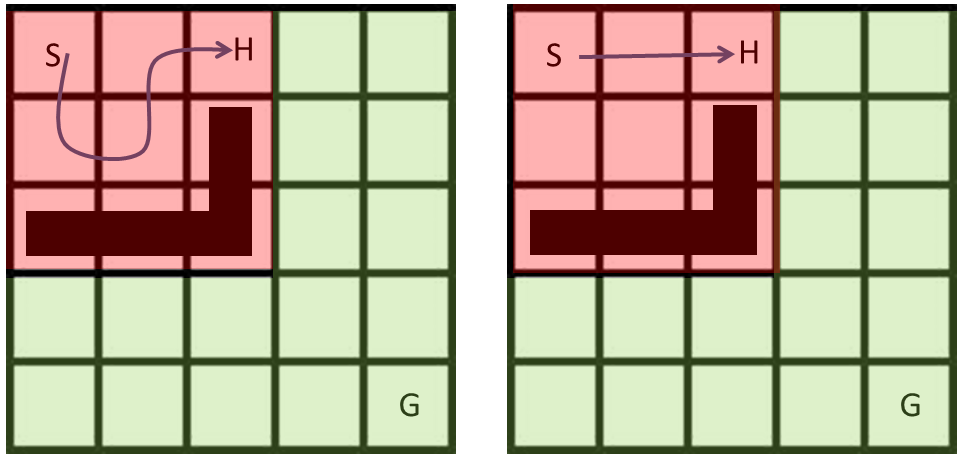
\includegraphics[width=2.7in]{fig/rsd_example.png}
  \caption{The two depicted LSP states $N$ (left) and $N`$ (right), where
  $N$ dominates $N`$ according to Theorem~\ref{the:rsd}.}
  \label{rsd_example}
\end{figure}

Figure~\ref{rsd_example} shows an example of two LSP states, $N$ (left) and $N`$ (right), that satisfy the dominance condition given in Theorem~\ref{the:rsd}.
The red areas represents the blocked vertices and green areas represents the reachable vertices.
As can be seen, both states have the same head,
the same sets of reachable states ($N.R=N`.R$),
and the length of $N.\pi$ is 4 while the length of $N`.\pi$ is 2. Thus, RDP will prune the state of the left.


%\Roni{There's some lack of symmetry. For BSD, we talked about implementation details. But here, no. Why?}
%\Yossi{Here we only use simple list we can say that since the visited area is not the same we can not hash therefore we need to compare more and this is the main downside of this method performance-wise}\AF{Then say that}

Implementing RDP in an efficient manner is a challenge, as it requires fast set inclusion computation. In our implementation, we used a simple linear search over the reachable states to check if one set of reachable states is included in the other. This indeed causes RDP to be sometimes slower than BSD, as can be seen in our experimental results.
%Here we only use simple list we can say that since the visited area is not the same we can not hash therefore we need to compare more and this is the main downside of this method performance-wise}\AF{Then say that}



\subsection{Pruning Dominated States During a Search}

\begin{algorithm}
\SetAlgoLined
    OPEN $\gets$ initial\\
    $g($initial$)\gets 0$\\
    CLOSED $\gets \emptyset$\\
    \While{OPEN is not empty}{
        $N\gets$ pop best state from OPEN\\
        Add $N$ to CLOSED\\
        \If{$N$ is a goal state}{
            \Return $N$
        }
        \ForEach{operator $o$ applicable in $N$ \nllabel{line:astar:for}}{
            $C\gets$ apply $o$ on $N$\\
            newg $C\gets$ $g(N)$+ cost($o$)\\
            %\If{$\exists$n$\in$OPEN$\cup$CLOSED s.t. Dominate(n,$g$(n), child, newg)}{
            \HiLi \If{$\exists N` \in$OPEN$\cup$CLOSED s.t. Dominate($N`$, $C$) \nllabel{line:astar:dominate1}}{
                \HiLi Goto line~\ref{line:astar:for}\\
            }
            %\ForEach{$n\in OPEN$ s.t. Dominate(child, newg, $n$, $g$(n))}{
            \HiLi \ForEach{$N`\in$OPEN s.t. Dominate($C$,$N`$)\nllabel{line:astar:dominate2}}{
                \HiLi Remove(N`, OPEN)
            }
            $g(C)\gets$newg\\
            Insert$\Big(C, g(C)+h(C)\Big)$ \nllabel{line:astar:insert}\\
        }
    }
    \Return no solution found
 \caption{The A* Algorithm}
 \label{alg:astar}
\end{algorithm}


Given a method for detecting dominated states we now describe how to use it in the context of A* and in the context of DFBnB.
We denote by \emph{Dominate(N,N`)} the application of the chosen dominance detection method. Algorithm~\ref{alg:astar} lists the pseudo-code for such an A* implementation. The highlighted lines are those that use the \emph{Dominate} method. When a child state $C$ is generated, we search for a state $N$ in OPEN or CLOSED that dominates $C$ (line~\ref{line:astar:dominate1} in Algorithm~\ref{alg:astar}). If such a state is found, then $C$ is not inserted into OPEN.
If there is no such dominating state in OPEN or CLOSED, we check if $C$ dominates a state $N$ that is already in OPEN (line~\ref{line:astar:dominate2}).
If this occurs, then $N$ is removed from OPEN. Finally,
$C$ is added to OPEN (line~\ref{line:astar:insert}).



To use BSD or RDP in DFBnB, we implemented DFBnB with a \emph{transposition table} that contains all generated states. Applying BDS for DFBnB is easy: prune a newly generated state if there exists a symmetric state in the transposition table.
The dominance relation detected by RDP is asymmetric, that is, one state dominates the other and not vice versa. Thus, pruning will only occur if DFBnB happened to generate the dominating state before the dominated states. This cuts down the effectiveness of RDP by half. Experimentally, this proved not cost-effective, and thus in our experimental results (Section~\ref{sec:experimental}) we only report results for DFBnB without any pruning and as well as with BSD only (but not with RDP).





\section{Heuristics}
\label{sec:heuristics}
In this section, we describe several admissible heuristic functions for solving LSP problems. %Recall that . Here, since this is a MAX problem, admissible means over estimation.

\subsection{The Reachable Heuristic}

For a state $N$, any graph-path that extends $N.\pi$ can never visit a vertex that is not in the reachable set of vertices. The \emph{Reachable} heuristic relies on this observation, denoted $h_{R}$
and defined as the size of the reachable set, i.e., $h_R(N)=|N.R|$. Clearly, $h_R$ is admissible.
The reachable heuristic will return 16 for both states in Figure~\ref{rsd_example}, as there are 16 reachable vertices (the green area).

To compute the reachable heuristic for a state $N$, we run a simple depth-first search starting from $N.head$ and spanning all reachable vertices.
The reachable heuristic was previously introduced by~\inlinecite{DBLP:conf/socs/SternKPFR14}.

\subsection{The Bi-Connected Components Heuristic}

\begin{figure}[ht!]
  \centering
  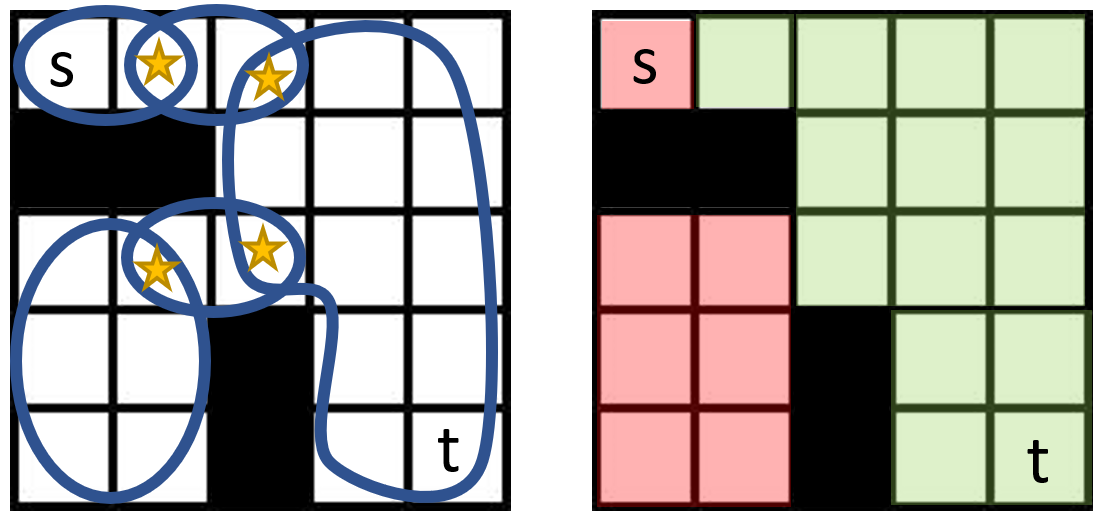
\includegraphics[width=3in]{fig/h_example_bcc2.png}
  \caption{An example of using the BCC heuristic. Left: the bi-connected components. Right: the vertices on the BCT branch that reaches the goal, marked in green.}
  \label{fig:h_example_bcc}
  %The figure on the left shows an LSP state in which the head is still in $s$, i.e., this is the initial state. The bi-connected components are marked with blue lines and the cut points with yellow pentagrams. The figure on the right marks in green the reachable states along the BCT branch that reaches the goal.}\label{fig:h_example_bcc}
\end{figure}
%\Yossi{Figure 3 caption is partly duplicated just before the "Alternate Steps Heuristic" subsection }

A bi-connected graph is a graph that remains connected after removing any single vertex. An equivalent definition is that every two vertices have at least two vertex-disjoint paths connecting them. A {\em bi-connected component} of a graph $G$ is a maximal sub-graph of $G$ that is bi-connected. A {\em cut-point} is a vertex that belongs to two different bi-connected components.
% Every graph can be decomposed to a BCT
Every graph can be decomposed into a set of biconnected components.
The resulting set of cut-points and bi-connected components form a {\em Block-Cutpoint-Tree} (BCT) that can be constructed in linear time~\cite{harary1966block,hopcroft1973algorithm}.
% Why do we care : only one branch counts

Two bi-connected components cannot have more than a single cut-point connecting them. Thus, once a graph-path passes a cut-point, it can never return to that bi-connected component.
Therefore, any simple graph-path passes through a single branch in the BCT.
In particular, any solution to an LSP problem must pass through the BCT branch that starts in the bi-connected component that contains $s$ and ends in the bi-connected component that contains $g$.
The {\em BCC} heuristic returns the sum of the number of reachable vertices in each of bi-connected component along this BCT branch, starting from the bi-connected component that contains the head of the evaluated state.  This heuristic is based on a similar heuristic proposed by Palmobo et al.~\shortcite{DBLP:conf/socs/PalomboSPFKR15} for the snake-in-the-box problem.


Figure~\ref{fig:h_example_bcc} shows an example of the BCC heuristic.
Figure~\ref{fig:h_example_bcc}(left) shows the initial LSP state, which represents an empty graph-path where the head is still in $s$. The BCT for this graph is visualized: bi-connected components are marked with blue lines and cut points with yellow stars.
Given this BCT, we can identify that the vertices on the bottom-left area are part of a bi-connected component that is not on the longest simple path from $s$ to $g$.
The vertices that are on the BCT branch that leads from $s$ to $g$ is marked in green in Figure~\ref{fig:h_example_bcc}(right). The BCC heuristic counts only these vertices, returning a value of 14. The reachable heuristic, will count all reach able states, returning 20 for this state.

\subsection{Alternate Steps Heuristic}

The following heuristic is applicable for cases where the underlying graph
represents a 4-connected grid, i.e., every grid cell is a vertex and there is an edge between this vertex and the vertices that represented its 4-connected neighboring grid cells.
%\Yossi{It will work not only on grids but on every bipartite graph, grid is one example and SIB is another domain that it applicable, In SIB the vertices with even number of ones can be white and odd number can be black }\Roni{Added a paragraph on this below}


Now, consider a grid marked like a board of chess, i.e., with grid cells are divided into black and white. A path along the board must alternate between white and black cells, that is,
if a vertex $v$ in a path is on a white cell then the next vertex in that path must be a black cell, and vice versa. For an LSP state $N$, let $\Delta$ be the difference between the number of white cells and black cells in the set of reachable vertices ($N.R$).
Assume the head of $N$ is a white cell. If the goal is a black cell, we can subtract $\Delta$ from the number reachable grid cells. If the goal is white cell, then we subtract $\Delta - 1$
from the number of reachable grid cells.
We denote by Reachable+alternate (R+ALT) the reachable heuristic enhanced with this method,
i.e., $h_{R+ALT}(N)=h_R(N)-\Delta$ of the head of $N$ and the goal are of the same color
and $h_{R+ALT}(N)=h_R(N)-\Delta+1$ otherwise.

%\Yossi{instead of "of the start and goal are of the same color" it should be "of the HEAD and goal are of the same color"}Fixed


\begin{center}
    \begin{table}[t]
    \begin{small}
    \setlength{\tabcolsep}{3pt}
    \centering
        \begin{tabular}{|c|r|r|r||r|r|}
       \hline
        & \multicolumn{3}{c||}{A*} & \multicolumn{2}{c|}{DFBnB}\\

        \thead{Heuristic} & \thead{NP} &  \thead{BSD} & \thead{RDP} & \thead{NP}  & \thead{BSD}  \\
        \hline
              R              & 92.5 &  97.5  & 91.4 & 100 & 100 \\
        \hline
              R+ALT        & 94.4 &  98.3  & 92.2 & 100 & 100 \\
        \hline
              BCC            & 99.4 &  100.0   & 99.7 & 100 & 100 \\
        \hline
              BCC+ALT       & 99.7 &  100.0   & 99.7 & 100 & 100 \\
        \hline
              BCC+S+ALT  & 99.7 &  100.0   & 99.7 & 100 & 100 \\
        \hline

        \end{tabular}
       %\caption{Success rate. Percentage of successfully solved \textit{Random Blocked Locations} problems within the 10 minutes time frame for every heuristic/pruning combination. From the total of 360 problems - most of the problems was solved.}
       \caption{Success rate, open grids with obstacles.}
    \label{tab:random_blocked_problems_solved_successfuly}
    \end{small}
    \end{table}
 \end{center}

\begin{center}
    \begin{table}[bt]
    \begin{small}
    \setlength{\tabcolsep}{3pt}
    \centering
        \begin{tabular}{ | c | r | r | r || r | r |}
        \hline
        & \multicolumn{3}{c||}{A*} & \multicolumn{2}{c|}{DFBnB}\\

        \thead{Heuristic} & \thead{NP} &  \thead{BSD} & \thead{RDP} & \thead{NP}  & \thead{BSD}  \\
        \hline
              R             & 45,211    & 21,815    & 16,494 & 49,772 & 24,823\\
        \hline
              R+ALT        & 34,271    & 15,708    & 14,051 & 38,100 & 18,286\\
        \hline
              BCC           & 8,366     & 2,703     & 2,271  & 9,623  & 3,447\\
        \hline
              BCC+ALT      & 7,491     & 2,187     & 2,077  & 8,651  & 2,869\\
        \hline
              BCC+S+ALT & 7,348     & 2,097     & {\bf 2,025}  & 8,499  & 2,771  \\
        \hline

        \end{tabular}
       %\caption{Average expanded nodes per heuristic and pruning method for all instances that have been solved by all configurations.}
       \caption{Average expanded states, open grids with obstacles.}
    \label{tab:expanded_nodes_comparison}
    \end{small}
    \end{table}
 \end{center}


%\Roni{Double check this}
%\Yossi{I think it should be:
%\\
%Assume the head of $N$ is a BLACK cell. If the goal is a black cell, we can subtract $\Delta$ from the number reachable grid cells. If the goal is white cell, then we subtract $\Delta - 1$ from the number of reachable grid cells.
%\\
%Because in the first case we our move sequence is W-B-W-B-W-B....-B - so the count must be the same. on the former scenario we get move sequence: W-B-W-B-W-B....-B-W  first and last are white so the white count should be one more than the black count}\AF{I think this is simple and we do not need this addition}


There are two ways to apply this enhancement on top of BCC. The first one is to apply it on the entire set of all vertices in all bi-connected components of the branch in the BCT. This is called BCC+ALT.
The second method is to apply this enhancement separately for each bi-connected component and then add them up. This is called BCC+separate+alternate (BCC+S+ALT).



%\section{BCC pruning by Preprocessing} \label{sec:bcc_pruning}

The BCC formulation can also be used to prune states. This is done by identifying in a preprocessing phase all the vertices that are not on the BCT branch leading to the goal vertex,
and considering all other vertices as blocked vertices. We found experimentally that doing this preprocessing proved beneficial, saving an average of 25\% of the number of expanded states, and saving approximately 30\% of the CPU time. Thus, we implemented this in all our variants and the experimental results included using this  method. %report below the resultwewe only report results below while using this method.
%\Roni{Yossi, please verify that the text above is correct}
%\Yossi{It is correct - actually on the random blocked grids I also have results without preprocessing but the presented results are only for preprocessing:ON. we are talking about an improvement to the reachable heuristic ONLY!. the improvement to BCC based heuristic was only in runtime and in avg. of around 3\%}



% Generality
This alternating heuristic, whether on top of the BCC heuristic or the Reachable heuristic, is more general than just for 4-connected grids. In fact, it is applicable for any underyling graph that can be represented as a bi-partite graph: the vertices on one part of the graph will be the ``black'' vertices and the vertices on the other will be the ``white'' vertices.

%%%%%%%%%%%%%%%%%%%%%%%%%%%%%%%%%%%%%%%%%%%%%%%%%%%%%%%%

\section{Experimental Results}
\label{sec:experimental}
In this section, we compared experimentally
A* and DFBnB using all the proposed pruning methods (no prunning, BSD, and RDP),
and heuristics (R, R+ALT, BCC, BCC+ALT, and BCC+S+ALT).
The underlying graphs used in our experiments are based on 4-connected grids.
Specifically, we used open grids with random obstacles and room map grids.



\subsection{Open Grids with Random Obstacles}

%The search space of LPP is exponential in the size of the map.
In this set of experiments we generated open grids with all integer combinations of sizes between 5x5 and 7x8 (total of 9 combinations). To each of these grids we set 4\%, 8\%, 12\% or 16\% cells as obstacles. For each of these percentiles we created 10 random LSP problems, yielding a total of 40 instance per gird size. In total, we had 360 random instances. A timeout of 10 minutes was set for solving each problem instance. %Every evaluated algorithm was
%All in all we had  360 random instances and we report results for these instances. We ran the solver with a time limitation of 10 minutes for every problem instance of the problem groups.

%%% TODO: Yossi - double check the RDP result (retry running it). - RDP couldnt solve in this time frame - checked!
%%% TODO: Yossi - add table that summarize the 80 instances of Big Rooms (running should finish today)  --- Merge with all rooms - total of 400 rooms


Table \ref{tab:random_blocked_problems_solved_successfuly} shows the \emph{success rate}, i.e., the percentage of instances (out of the 360 available problems) that were solved within the 10 minute limit. The rows are the different heuristics and the columns are the different search algorithms coupled with the different pruning techniques.
We denoted by ``NP'' the columns that represent not using any pruning technique. This table shows that DFBnB
and A*+BSD using any of the BCC heuristics are able to solve all the problem instances.
%solved more instances than A* and that the algorithms perform better as we have more sophisticated heuristics and more advanced pruning techniques. [[AF: Yossi claims that the number are not final. Why is BSD better than RDP which is more sophisticated.]






\begin{center}
    \begin{table}[bt]
    \centering
    \begin{small}
    \setlength{\tabcolsep}{3pt}
        \begin{tabular}{ | c | r | r | r | r | r |}
        \hline
        & \multicolumn{3}{c|}{A*} & \multicolumn{2}{c|}{DFBnB}\\

        \thead{Heuristic} & \thead{NP} &  \thead{BSD} & \thead{RDP} & \thead{NP}  & \thead{BSD}  \\
        \hline
              R                  & 10,808 &  2,626 & 17,576 & 601 & 448  \\
        \hline
              R+ALT             & 6,155  &  1,417 & 14,386 & 463 & 338 \\
        \hline
              BCC                & 377    &  110   & 294    & 195 & 105 \\
        \hline
              BCC+ALT           & 300    &  {\bf 82}    & 262    & 150 & 86 \\
        \hline
              BCC+S+ALT      & 311    &  86    & 261    & 149 & 94 \\
        \hline

        \end{tabular}
        \caption{Average runtime (ms), open grids with obstacles.}
       %\caption{Average runtime (ms), open grids per heuristic and pruning method for all instances that have been solved by all configurations.}
    \label{tab:runtime_comparison}
    \end{small}
    \end{table}
 \end{center}




Table \ref{tab:expanded_nodes_comparison} compares the number of expanded states per solver averaged over all instances that could be solved by all methods.
The main expected trends are very clear. First, the more advanced heuristics yielded fewer state expansions. The main advantage comes from using the BCC heuristics,
as the differences between the BCC heuristics is quite small. Second, RDP is able to prune more states than BSD, and BSD prunes a significant number of states (when compared to NP).
Note that the best method of A*+RDP with the BCC+S+ALT heuristic is better than the baseline A* variant by a factor of 22.
Table \ref{tab:runtime_comparison} gives similar results but for runtime in milliseconds.
Here, we see that the RDP was slower than the BSD method, although it expanded fewer states.
This is reasonable since RDP incurs a large CPU overhead. Neverthelss, when considering the best method (A*+BSD), it is 12 times faster than the baseline A* variant (no prunning, reachable heuristic).





 \subsection{Room Maps}


\begin{center}
    \begin{table}[bt]
    \begin{small}
    \setlength{\tabcolsep}{3pt}
    \centering
        \begin{tabular}{ | c | r | r | r || r | r |}
        \hline
        & \multicolumn{3}{c||}{A*} & \multicolumn{2}{c|}{DFBnB}\\

        \thead{Heuristic} & \thead{NP} &  \thead{BSD} & \thead{RDP} & \thead{NP}  & \thead{BSD}  \\
        \hline
              R             & 58.3 & 62.5 & 72.0  & 68.5 & 70.0 \\
        \hline
              R+ALT         & 61.3 & 65.0 & 72.8  & 70.5 & 71.3 \\
        \hline
              BCC           & 72.0 & 76.0 & 81.5  & 76.0 & 78.0 \\
        \hline
              BCC+ALT       & 74.0 & 77.8 & 81.5  & 77.0 & 79.0 \\
        \hline
              BCC+S+ALT     & 75.3 & 79.8 & \textbf{82.3}  & 78.5 & 80.3 \\
        \hline


        \end{tabular}
       %\caption{Percentage of successfully solved \textit{Room Maps} problems within the 10 minutes time frame for every heuristic/pruning combination out of 400 instances.}
\caption{Success rate, room maps.}% runtime (ms), open grids with obstacles.}

    \label{tab:rooms_problems_solved_successfuly}
    \end{small}
    \end{table}
 \end{center}

\definecolor{bblue}{HTML}{4F81BD}
\definecolor{rred}{HTML}{C0504D}
\definecolor{ggreen}{HTML}{9BBB59}
\definecolor{ppurple}{HTML}{9F4C7C}


\begin{figure*}[bt]
\centering

\begin{subfigure}{.3\linewidth}
            \centering

\begin{tikzpicture}
    \begin{axis}[
        width  = 1*\textwidth,
        height = 6cm,
        major x tick style = transparent,
        ybar=2*\pgflinewidth,
        bar width=6pt,
        ymajorgrids = true,
        ylabel = {Expanded states},
        symbolic x coords= {R,R+ALT,BCC, BCC+ALT, BCC+S+ALT},
        % x tick label style = {font = \footnotesize, text width = 2cm, rotate = -40, anchor = north west},
        x tick label style={rotate=45, anchor=east, align=right,text width=2cm},
        xtick = data,
        scaled y ticks = false,
        ylabel near ticks,
        enlarge x limits=0.15,
        ymin=0,
        legend cell align=left,
        % legend style={
        %         at={(1,1.01)},
        %         anchor=south east,
        %         column sep=1ex
        % }
    ]
        \addplot[style={bblue,fill=bblue,mark=none}]
            coordinates {(R, 30477) (R+ALT,23865) (BCC,10935) (BCC+ALT,8731) (BCC+S+ALT,6135)};

         \addplot[style={rred,fill=rred,mark=none}]
            coordinates {(R, 18658) (R+ALT,13817) (BCC,5577) (BCC+ALT,4063) (BCC+S+ALT,2326)};

        \addplot[style={ggreen,fill=ggreen,mark=none}]
            coordinates {(R, 3549) (R+ALT,3324) (BCC,1618) (BCC+ALT,1516) (BCC+S+ALT,1433)};

        \legend{No pruning,BSD,RDP}
    \end{axis}
\end{tikzpicture}


        \caption{Average expanded states, A*.}
        \label{chart:rooms_expanded_a_star}
    \end{subfigure}%
    \hfill%
    \begin{subfigure}{.27\linewidth}
        \centering
        \begin{tikzpicture}
            \begin{axis}[
                width  = 1*\textwidth,
                height = 6cm,
                major x tick style = transparent,
                ybar=2*\pgflinewidth,
                bar width=8pt,
                ymajorgrids = true,
                ylabel = {Expanded states},
                symbolic x coords= {R,R+ALT,BCC,BCC+ALT, BCC+S+ALT},
                % x tick label style = {font = \footnotesize, text width = 2cm, rotate = -40, anchor = north west},
                x tick label style={rotate=45, anchor=east, align=right,text width=2cm},
                xtick = data,
                scaled y ticks = false,
                ylabel near ticks,
                enlarge x limits=0.15,
                ymin=0,
                legend cell align=left,
            ]
                \addplot[style={bblue,fill=bblue,mark=none}]
                    coordinates {(R, 74987) (R+ALT,62534) (BCC,34059) (BCC+ALT,29114) (BCC+S+ALT,22047)};

                 \addplot[style={rred,fill=rred,mark=none}]
                    coordinates {(R, 41726) (R+ALT,32201) (BCC,17428) (BCC+ALT,13679) (BCC+S+ALT,9020)};

                \legend{No pruning,BSD}
            \end{axis}
        \end{tikzpicture}
        \caption{Average expanded states, DFBnB.}
        \label{chart:rooms_expanded_dfbnb}


    \end{subfigure}
    \hfill
    \begin{subfigure}{.4\linewidth}
        \centering

        \begin{tikzpicture}
            \begin{axis}[
                width  = 1*\textwidth,
                height = 6cm,
                major x tick style = transparent,
                ybar=2*\pgflinewidth,
                bar width=7pt,
                ymajorgrids = true,
                ylabel = {Average runtime (ms)},
                symbolic x coords= { A* BCC, A* BCC+ALT, A* BCC+S+ALT, BnB BCC, BnB BCC+ALT, BnB BCC+S+ALT},
                % x tick label style = {font = \footnotesize, text width = 2cm, rotate = -90, anchor = north west},
                x tick label style={rotate=45, anchor=east, align=right,text width=2cm},
                xtick = data,
                scaled y ticks = false,
                ylabel near ticks,
                enlarge x limits=0.1,
                ymin=0,
                legend cell align=left,
                legend style={
                        at={(0.01,0.65)},
                        anchor=south west,
                        column sep=1ex
                }
            ]
                \addplot[style={bblue,fill=bblue,mark=none}]
                    coordinates {(A* BCC, 1400) (A* BCC+ALT,1090) (A* BCC+S+ALT,596) (BnB BCC,2619) (BnB BCC+ALT,2113) (BnB BCC+S+ALT, 1295) };

                \addplot[style={rred,fill=rred,mark=none}]
                    coordinates {(A* BCC, 714) (A* BCC+ALT,512) (A* BCC+S+ALT,222) (BnB BCC,1789) (BnB BCC+ALT,1344) (BnB BCC+S+ALT, 732) };

                \addplot[style={ggreen,fill=ggreen,mark=none}]
                    coordinates {(A* BCC, 1069) (A* BCC+ALT,1008) (A* BCC+S+ALT,1005)   };
                \legend{No pruning, BSD, RDP}
            \end{axis}
        \end{tikzpicture}

        %removedVspace
        \caption{Average runtime, A* and DFBnB.}
        \label{chart:rooms_runtime}
    \end{subfigure}

    \caption{Room maps result charts, all comparisons are for instances that was were solved by all algorithms, heuristics and pruning}
\end{figure*}
%\Yossi{Notice: I've added to chart 4 -"all comparisons are for instances that was were solved by all algorithms, heuristics and pruning" }



 For this set of experiments, we generated grids shaped like a house with rooms.
 Every grid contains multiple rooms connected via narrow \textit{doors}, the doors are randomly positioned. % and we randomly decide if the door is open or closed. IF IT IS CLOSED THEN IT IS NOT A DOOR
 The number of rooms in a grid varies between 3x2 and 5x6, where the room size was between 2x2 and 5x5. %, in order to keep the problems somehow solvable we have used smaller room sizes with bigger grids.
 400 such room maps were created for our experiments.
 Table \ref{tab:rooms_problems_solved_successfuly} shows the success rate of the different LSP algorithms on this type of grids.
 In this domain, the A*+RDP method outperforms all other methods, but DFBnB+BSD provides comparable results.
 % Also here we can examine close performance between  A* + RDP and DFBnB + BSD with a slight advantage to the former.Unlike in the {\em Random Blocked Locations} problems set that some of the algorithm -- pruning method was solved by all heuristics in this problem set we can see that for every pruning method and algorithm combination there is a consistent order on the heuristic effectiveness (bigger means more effective heuristic - solve more problems) R $\leq$ R+ALT  $\leq$ BCC $\leq$ BCC+ALT $\leq$ BCC+S+ALT,
 The observed trends here are that indeed stronger heuristic and stronger pruning method yielded higher success rate.


Similar trends are observed when considering the number of expanded states and runtime. Figures \ref{chart:rooms_expanded_a_star} and Figure \ref{chart:rooms_expanded_dfbnb} plots the average number of expanded states for the different pruning methods and heuristics
for A* and for DFBnB, respectively. The impcat of using both pruning and heuristics is very clear: RDP provides more pruning compared to BDS, which in terms provides more pruning compared to not performing any pruning. A comparison of the run-times over instances solved by all appears in \ref{chart:rooms_runtime}. The results show a more complex picture, where the overhead of using RPD is not worthwhile in terms of runtime. BSD provides a good balance in this domain, of runtime overhead and strength of the chosen dominating systems.



To summarize, we observe the following. First, the BCC heuristic is always better than Reachable.
Second, adding the alternating step on top of the BCC heuristic is helpful, but not by a large margin.
Third, it is always worthwhile to perform the BSD prunning. The RDP pruning always saves state expansions, but its runtime is sometimes worst than that of BSD.
Forth, when comparing DFBnB to A*, we observe that their performance is usually quite similar, when equipped with a good heuristic.




\section{Conclusion and Future Work}

In this paper we proposed several techniques to help solve the longest simple path problem. These techniques include
methods for pruning states that are dominated by other states, and a range of admissible heuristics. We explain how to use these pruning methods and heuristics in two popular search algorithms: A* and DFBnB.
We evaluted the impact of each of the newly proposed techniques experimentally on two types of grid maps. The results show that the proposed pruning methods and heuristics improves the ability to solve LSP problems in reasonable time.
%\\ We have shown that the BCC pre-processing step is very useful since it decrease the search time for any solver configuration (algorithm/heuristic/pruning) especially for the non-bcc based heuristics. \\ Different than the conclusions appear in \cite{DBLP:conf/socs/PalomboSPFKR15} we have shown here that DFBnB not always performs better than A* on a various heuristics and pruning combinations.\\ We have shown that the BSD pruning with hash function is the most effective pruning method w.r.t run-time and that the RDP is the most effective pruning method w.r.t expanded nodes.
% \\

This work opens several compelling directions for future work. First, we focused on finding an optimal solution to LSP. Future work can explore how to tradeoff optimality for runtime.
%finding sub-optimal solutions faster.  More research still need to be made in this field, This work didn't cover the sub optimal aspect of LPP. This aspect is sure need further research, In the GitHub \cite{Yossico2019} project that was implemented as part of this thesis there is also a greedy algorithm implementation, It will be nice if someone will pick up the glove and use this open source project to research the sub optimal area of LPP.
%\\
The suggested pruning methods, and in particular RDP, can be time consuming. Future work may develop more efficient data structures that will allow fast searching of dominated states. %inclusi that is used for comparing the search nodes, As we introduced before, simple hashing improved BSD performance. Similar improvement can be researched for RSD w.r.t the visited area and the reachable area. RSD has a huge potential since it prunes better then all other pruning methods and a better data structure that will cut off the times probably will make it better than BSD in all aspects.
%\\
%We hope that this work will help other researches that needs to solve LPP from real world scenarios.



Praesentium commodi nemo id ullam voluptatibus perferendis officiis officia, sed harum repudiandae, ullam exercitationem a assumenda nulla expedita reprehenderit sequi, mollitia recusandae fuga alias quisquam nisi corrupti consectetur atque incidunt delectus reprehenderit?Corrupti adipisci dolorem delectus voluptas assumenda aspernatur, quae numquam distinctio eligendi autem nisi minima quos?Praesentium earum tenetur velit voluptates nostrum illum quisquam unde iste quidem corporis, minima voluptas fugit inventore illum dignissimos quidem quo rerum nam, excepturi illum atque ratione assumenda provident impedit hic, dolorum quas corporis quibusdam sit amet ea reiciendis nesciunt maxime.Neque quaerat obcaecati omnis dolores ab dignissimos quo libero cupiditate illo, ullam officiis nemo maxime laudantium fuga tempora, iste nulla at reprehenderit enim eius vitae dolorem, veritatis fugiat ducimus, minima hic ut non velit mollitia minus magni nostrum recusandae possimus molestias?Ut ad dolorum temporibus itaque consequatur, eligendi consequatur ad harum ratione error veritatis est fuga nisi enim, eveniet quo necessitatibus repellendus.Ipsum dolores dignissimos rem atque est magni voluptates, ab tenetur molestias nobis consectetur incidunt aperiam corrupti assumenda cumque nulla, commodi distinctio dignissimos pariatur quam architecto voluptatum esse quisquam.Voluptatibus cum optio, veniam distinctio et nihil esse incidunt modi provident aliquam ipsa omnis ab, fugit eaque ea corporis dolorem, dolorum fugit possimus ex assumenda dolor, tempore facilis fugit facere perferendis accusantium.Molestias perspiciatis impedit nam velit deleniti optio, esse voluptatibus dignissimos modi incidunt expedita asperiores, veritatis ipsam sapiente facere aliquid temporibus minima illum inventore nisi nostrum iure dolorem, rerum voluptate ipsa voluptatem alias quasi et sint voluptatum?Rem quas enim pariatur animi magni quaerat doloribus facere, libero incidunt ut nihil expedita obcaecati ex adipisci laborum necessitatibus vel.Vero laudantium dignissimos corporis illo natus adipisci, facere assumenda provident porro eos iusto?Maiores fugiat officiis eius, dolorem labore harum accusantium nesciunt ducimus nisi quisquam aut optio, harum rerum doloremque velit voluptas dolorum minima similique nesciunt dignissimos deleniti, excepturi aspernatur eveniet omnis numquam eos, maiores ex eius?Odit impedit aliquid debitis eligendi alias dolore ullam accusantium in, voluptate error inventore atque saepe aperiam ipsa impedit, fugiat illum explicabo et sed vero esse doloremque eos debitis, aliquam alias commodi officiis hic inventore quidem ratione laudantium.Consequuntur aperiam dicta sunt soluta, repellat eaque odio officiis quaerat nihil iure, corrupti blanditiis beatae similique officiis nisi ullam autem sed, doloribus perspiciatis ducimus necessitatibus quisquam modi qui autem repellendus maxime labore, sapiente inventore suscipit id repudiandae illum provident debitis quos?Cupiditate eius possimus, id cupiditate ducimus quod?Nam aliquid quaerat reiciendis quam corrupti, sed autem itaque maxime.Consequuntur libero molestias optio recusandae nam saepe, explicabo exercitationem voluptates ipsa blanditiis modi est nemo voluptas sint, fuga dicta numquam expedita illo porro doloribus beatae adipisci consequuntur.Fugiat earum eveniet est, soluta nobis deserunt dolore ipsa ad voluptates inventore architecto molestias, nostrum maxime quas esse.Et atque velit beatae laudantium illo ut dolorem consequatur, velit consectetur dolorem iusto excepturi amet consequatur quam, esse tempore nemo quasi, tenetur voluptatibus ab amet nam vero voluptates molestiae eveniet nisi sapiente dolore, sequi laborum placeat atque perferendis iure nesciunt vero quo illo modi  aperiam natus cupiditate ratione quas exercitationem laudantium et quae, vitae odit architecto, qui ea aliquam, excepturi fugit dolores vero aspernatur.\clearpage
\bibliography{thesis}
\bibliographystyle{aaai}
\end{document}